%%%%%%%%%%%%%%%%%%%%%%%%%%%%%%%%%%%%%%%%%%%%%
%%%%%%%%%%%%%%%%%%%%%%%%%%%%%%%%%%%%%%%%%%%%%
%%%%%%%%%%%%%%%%%%%%%%%%%%%%%%%%%%%%%%%%%%%%%

\section{The International Linear Collider}
\subsection{Role in particle physics}
Particle accelerators, that produce colliding beams, colliders, drive the progress of our understanding of the subatomic world.

For particle physics, two types of colliders are relevant:
\begin{itemize}
\item Hadron colliders have beams of proton and/or antiproton, for example SppS, TeVatron or LHC;
\item Lepton colliders collide electron and positron beams, for example SLC, PETRA or LEP.
\end{itemize}

%The hadron colliders are generally considered as a "discovery" machines due to their higher center-of-mass energy, while electron-positron colliders mostly used for a consolidation of theoretical conclusions by high-precision measurement of theory parameters. 
%LHC is great 

The Large Hadron Collider is the most powerful proton-proton collider made and it has already made a breakthrough by discovering the Higgs boson.  Nevertheless, to measure precisely all accessible properties of the Higgs particle and other \sm\ particles scientific community needs a new high-precision experiment.

It is a worldwide consensus, that the next large high-energy physics facility after LHC should be a lepton collider. 
The main advantages of a lepton collider over hadron machines are a well-known initial state of colliding particles and a higher signal to background ratio for many physics processes.
The linear electron-positron colliders, like SLC at Stanford, have higher energy reach, more focused beams having more compact accelerator complex, than equivalent circular machines.

The International Linear Collider is a project of linear electron-positron collider designed for energies between 250\,GeV and 1000\,TeV. 
The Compact Linear Collider (CLIC) is an alternative project of a future electron-positron machine with nominal $\sqrt s$ of 3\,TeV. 
This thesis is focused on ILC project.
%Its parameters have been set by physics requirements and reviewed continuously by a wide scientific community. The R\&D was summarized in the Technical Design Report (TDR).~\cite{bib:ILC}
The ILC is designed for searches of New Physics and high-precision measurements of the crucial \sm\  parameters. 
The ILC physics program is oriented on the production thresholds of heavy \sm\ particles the Higgs and the top quark. 
The physics potential of the ILC project will be enhanced by polarized beams, which can be used to suppress background processes in electroweak physics. 


%According to these features, the ILC has a rich physics program, precision measurements of the \sm\ parameters, as well as direct and indirect searches of New Physics. 
%%%%%%%%%%%%%%%%%%%%%%%%%%%%%%%%%%%%%%%%%%%%%
%%%%%%%%%%%%%%%%%%%%%%%%%%%%%%%%%%%%%%%%%%%%%
%%%%%%%%%%%%%%%%%%%%%%%%%%%%%%%%%%%%%%%%%%%%%


\subsection{Research program at the International Linear Collider}

Following the discovery of the Higgs boson by the LHC experiments, the ILC will complement the LHC discovery by measuring precisely all accessible properties of this particle.
The main advantage of the ILC is a model-independent measurement of the Higgs properties by studying  the Higgs-strahlung $e^+e^-\to Z^0H$ process, and measurement of full width of Higgs decay, which is impossible at the LHC experiments. 

%No information on the BSM
%ILC is an ideal machine to look for invisible Higgs decays or light dark matter searches, due to its high detector hermeticity. 

%The ILC has highly polarized beams, flexible center-of-mass energy and high-granular detectors, which makes it a perfect machine for studying of electroweak processes, as well as many others. 

%The nominal center-of-mass energy of the ILC is 500\,GeV, which can be increased up to 1\,TeV. 
The ILC can run at the center-of-mass energy of 250\,GeV, which gives the peak production for the  Higgs-strahlung reaction. 
The top mass can be precisely measured at 350\,GeV energy, at the top pair production threshold. 
The couplings of the Higgs and top particles can be studied at 500\,GeV, as well as at 1\,TeV center-of-mass energy.
Therefore, the physics program covers several important thresholds in the \sm\ physics, that are summarized in Table~\ref{table:SMILCmeasurements}. 


\begin{table}[H]
\centering

\begin{tabular}{@{}rll@{}}
\toprule
Energy & Process & Goal of measurements\\ 
\midrule

91\,GeV  & $e^+e^- \to Z^0$  		& $Z^0$ physics and calibration \\
250\,GeV & $e^+e^- \to Z^0H$  		& Higgs couplings \\
		 & $e^+e^- \to f\bar{f}$  	& $Z^0/\gamma$ couplings \\
350\,GeV & $e^+e^- \to t\bar{t}$ 	& top mass precision \\
		 & $e^+e^- \to \nu\bar{\nu}H$ & Higgs couplings \\
500\,GeV & $e^+e^- \to t\bar{t}$ 	& top couplings \\
 		 & $e^+e^- \to t\bar{t}H$ 	& Higgs-top coupling \\ 
 		 & $e^+e^- \to Z^0HH$ 		& Higgs self coupling \\ 
1000\,GeV & $e^+e^- \to \nu\bar{\nu}HH$&  Higgs self coupling \\
 \bottomrule
\end{tabular}

\caption{\sl Major \sm\ processes to be studied at ILC. \cite{bib:ILC}}
\label{table:SMILCmeasurements}
\end{table}

%SM is a chiral theory 
Polarized beams of the ILC deliver a more detailed information on the \sm\ coupling constants, and more control over background process rates. 
The variable center-of-mass energy of the collisions will provide an information on energy dependence of many important \sm\ parameters. 
 
The ILC will resolve the ambiguities of the \sm\ electroweak fit, displayed in Fig.~\ref{fig:SM3deviations}, in a clear and definite way. 

%top
%Along with the Higgs boson, the top quark has never been studied in electroweak environment of electron-positron colliders. 
%The access to the electroweak coupling constant of the top quark is limited for hadron colliders, while the ILC can measure these values to a percent precision.

Besides the \sm\ precision measurements, the ILC has a rich program of New Physics searches. 
There are huge variety of studies made by ILC community, dedicated to the direct searches of the dark matter, additional particles from supersymmetric theories, indirect searches of resonances from extradimentional models, etc.

%The production of the top quark for the hadronic machines, like TeVatron or LHC, is via the gluon splitting, while at the ILC, the dominant top quark production is
% 3 important thresholds ZH, tt, ZHH
% beam polarisation 
\subsubsection{Operating scenarios of the ILC}
\label{sec:ILCOperation}
The ILC running scenarios are described in report~\cite{bib:H20}. 
The preferable running option is called H-20, which is optimized to reach the desired accuracies on the \sm\ couplings during 20 years of ILC operation time. 
The accumulation of the integrated luminosity with time in this scenario is shown in Fig.~\ref{fig:H20}.
The foreseen luminosity upgrade of the accelerator complex~\cite{bib:LumiUp} allow to significantly increase the collision event rate. 

\begin{figure}
	{\centering
		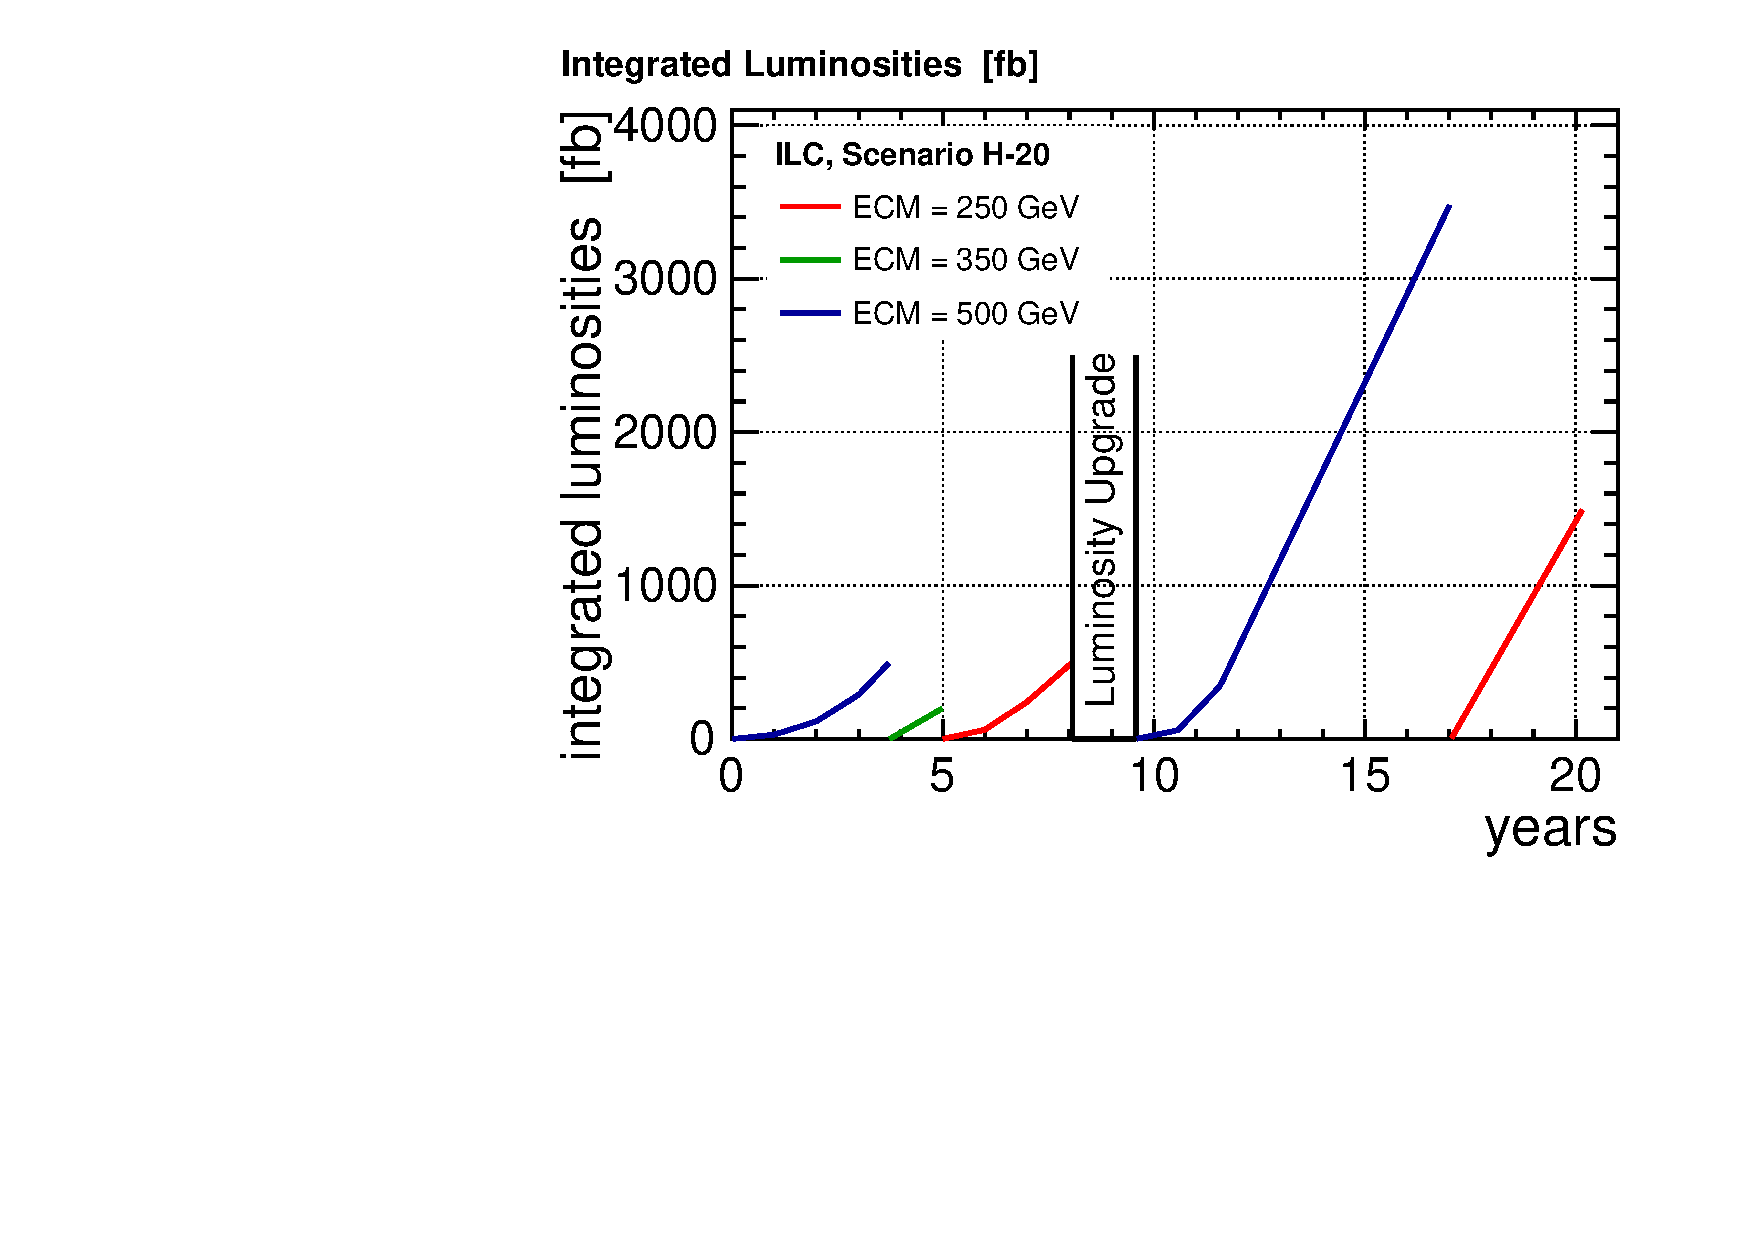
\includegraphics[width=0.55\textwidth]{graphics/lumi_H-20.pdf}
		\caption{\sl Accumulation of integrated luminosity versus real time in calendar years for scenario H-20.}
		\label{fig:H20}
	}
\end{figure}
In the H-20 scenario, the ILC physics program starts directly from 500\,GeV center-of-mass energy by collecting 500\ifb\ integrated luminosity. This choice makes possible to study all \sm\ processes from the beginning of the ILC physics operation.
The ILC will collect 500\ifb\ integrated luminosity at $\sqrt{s} = 250$\,GeV before the luminosity upgrade.
The luminosity sharing between different beam polarizations are described in Table~\ref{tab:H20}. 

\begin{table}[h]
\centering
  \renewcommand{\arraystretch}{1.10}
\begin{tabularx}{\textwidth}{*{5}{>{\centering\arraybackslash}X}}    %\begin{tabular*}{\textwidth}{@{\extracolsep{\fill}}|c|c|c|c|c|}
%\begin{tabular}{|l|c|c|c|c|}
\hline
        &  \multicolumn{4}{c}{integrated luminosity with $\operatorname{sgn}(P(e^-),P(e^+))= $ } \\
           & (-,+)       & (+,-)       & (-,-)       &  (+,+)     \\
\hline
$\sqrt{s}$ & [fb$^{-1}$] & [fb$^{-1}$] &  [fb$^{-1}$] & [fb$^{-1}$] \\ 
\hline
250\,GeV    &  1350      &  450        &  100	      &   100  \\
350\,GeV    &   135      &   45	       &   10	      &    10  \\
500\,GeV    &  1600      & 1600        &  400	      &   400  \\
\hline
\end{tabularx}
\caption{Integrated luminosities per beam helicity configuration in scenario H-20~\cite{bib:H20}.
}
\label{tab:H20} 
\end{table}
%%%%%%%%%%%%%%%%%%%%%%%%%%%%%%%%%%%%%%%%%%%%%
%%%%%%%%%%%%%%%%%%%%%%%%%%%%%%%%%%%%%%%%%%%%%
%%%%%%%%%%%%%%%%%%%%%%%%%%%%%%%%%%%%%%%%%%%%%

\subsection{Accelerator complex}
Electrons and positrons are the lightest charged particles, therefore they have preference to emit a synchrotron radiation in a magnetic field. For circular accelerators the synchrotron radiation $E_{rad}$ strongly depends on the radius of accelerator $r$, particle mass $m$ and particle energy $E$ as
\begin{equation}
	E_{rad} \propto \frac{E^4}{m^4r}.
\end{equation}
This is the main limitation of circular electron-positron colliders, where dipole magnets of their accelerator system cause strong beam energy losses. 
The linear accelerator design avoid these complications and allow production and analysis of high energy collisions. 

%CHANGE !!!!!!!!!!!
However, the linear accelerator design present many challenges: high acceleration gradients are required to achieve the full beam energy in a single pass and the beams must have a high intensity and be focused to a small spotsizes to achieve high collision rates, since the beams intersect only once.
% synchrotron radiation
% Years of R&D 

The schematic view of the entire accelerator system in  Fig.~\ref{fig:ILCScheme}. 
\begin{figure}
{\centering
    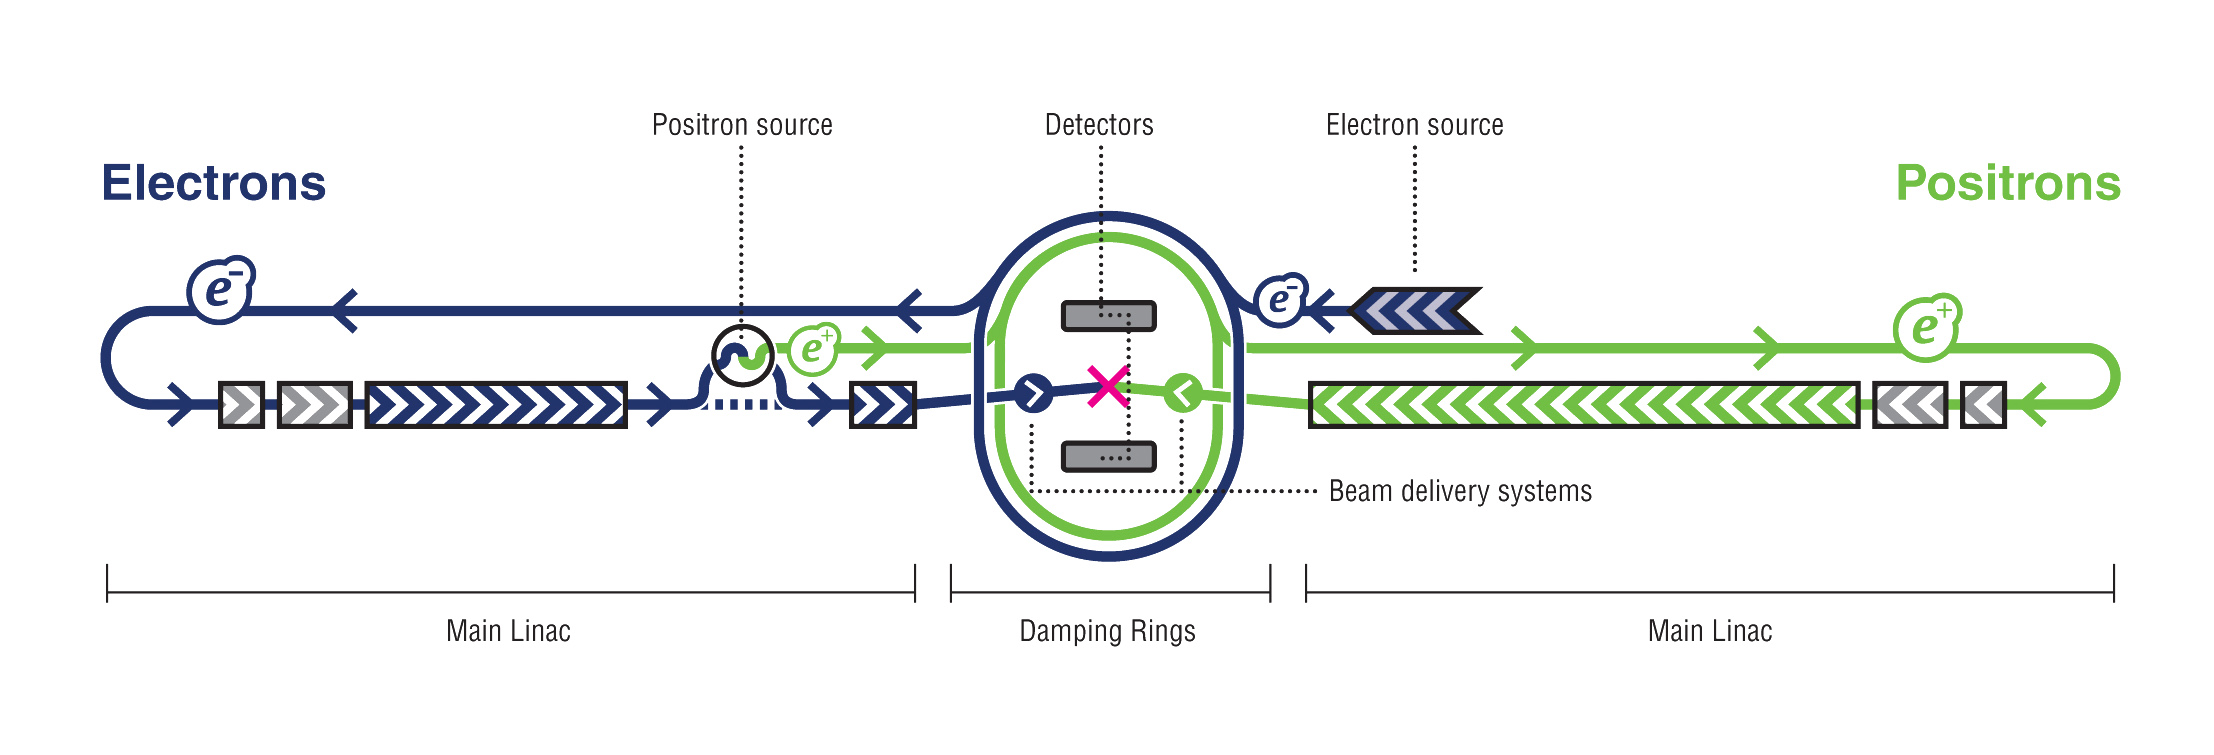
\includegraphics[width=0.95\textwidth]{graphics/ILC_scheme.jpg}
    \caption{\sl Schematic view of the ILC accelerator complex.}
    \label{fig:ILCScheme}
  }
\end{figure}
The ILC accelerator complex is the result of more than a decade of a detailed research and development. 
The major sub-systems of the ILC accelerator are:
\begin{itemize}
\item a photocathode DC gun as polarized electron source
\item an undulator on the main electron beam accelerator as a polarized positron source
\item 5\,GeV electron and positron dumping rings to reduce a phase space of the initial particles
\item positron and electron 11\,km linear accelerators or linacs, composed of 1.3\,GHz cavities
\item a beam delivery system to bring the beams to the interaction point, which is shared by two detectors with push-pull configuration.
\end{itemize}
The main parameters of the beams, produced by the linac complex are given in Table~\ref{tab:ILCparam}.

\textit{The polarized electron beam} is obtained by sending a laser beam on a strained superlattice GaAs cathode which emits a bunch of electrons with high polarization. Then, the electrons are accelerated to 5\,GeV and injected into the electron damping ring.

\textit{The polarized positrons} are obtained by selecting positrons from $e^+ e^-$ pairs, created by converting polarized high energy photons on a rotating Ti-alloy target. The polarized photons are radiated by passing electrons in a superconducting helical undulator on the main electron beam.
A detailed layout of positron source is shown in Fig.~\ref{fig:ILCeplus}.
Similar to the electrons, the positron beam is accelerated to 5\,GeV energy in a superconducting linac before injection into the positron dumping ring. 

\begin{figure}
{\centering
    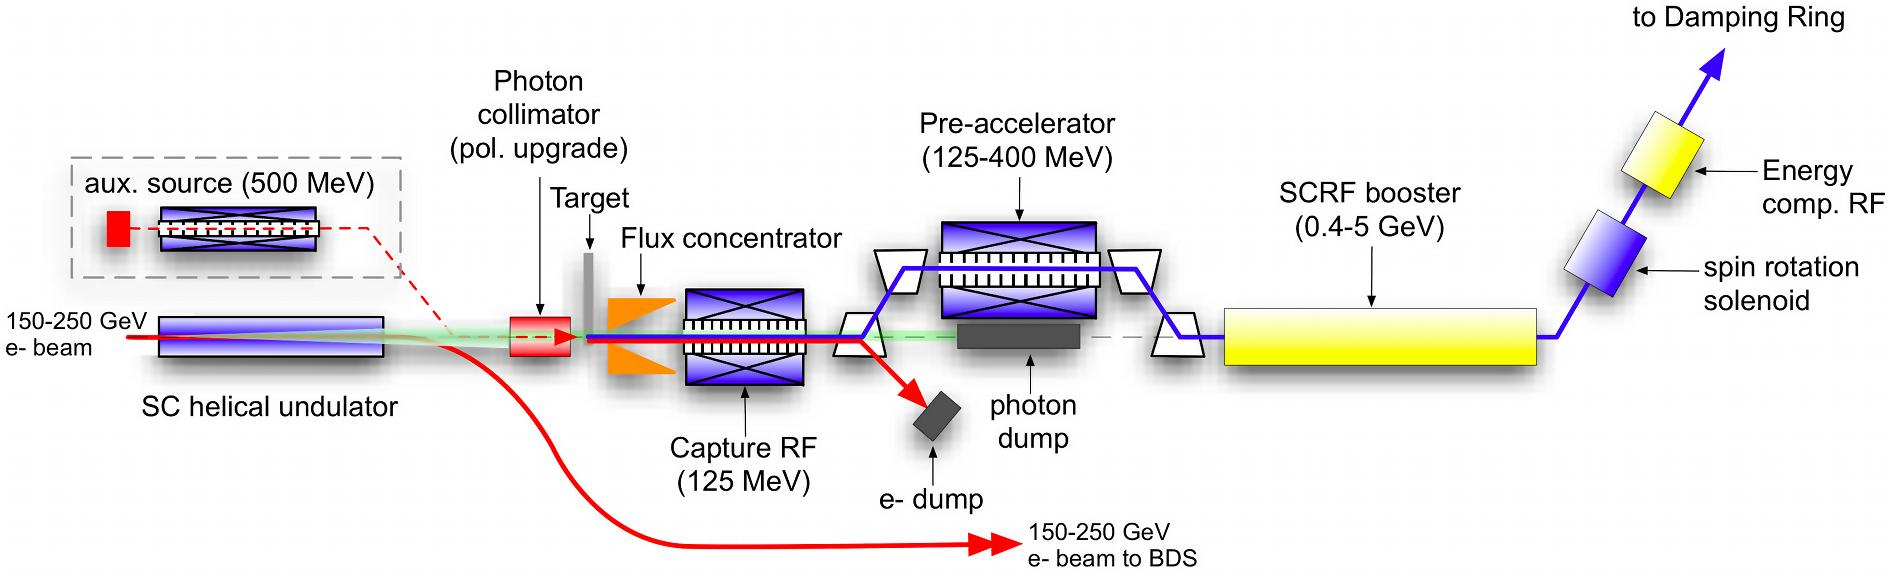
\includegraphics[width=0.95\textwidth]{graphics/ILCeplus.jpg}
    \caption{\sl Schematic view of the ILC positron source.}
    \label{fig:ILCeplus}
  }
\end{figure}

\textit{The damping rings} are housed in a common tunnel with circumference of 3.2\,km. They accept electrons and positrons with large transverse and longitudinal emittances and damp them to the low emittances needed for injection into the main linac. 
Each damping ring accommodates the injection and extraction systems, RF cavities and dumping wigglers.
The damping is made by an array of superferric wigglers in both dumping rings, which operate at 4.2\,K with 2.16\,T magnetic field. 
Both damping rings are connected to the main linear accelerators by transfer lines.

\textit{The main linear accelerators} are designed to accelerate the particles from 15\,GeV to a nominal energy of 250\,GeV. 
The acceleration is provided by approximately 7400 superconducting radio-frequency nine-cell niobium cavities (see Fig.~\ref{fig:ILCcavity}) operating at 2\,K temperature. 
The baseline accelerating gradient of the cavities is 31.5\,MV/m. 
The industrial mass production of the cavities can cause a random gradient variation of $\pm$20\%. 
The balance between key parameters is a result of years of intensive R\&D by a wide scientific community. 
The cavities are assembled into two types of cryomodules: type A with nine SCRF cavities and type B with eight SCRF cavities and one superconducting quadrupole magnet located at the center of the module. 
The technology of industrial production of the cavities for ILC is a great challenge and there is room for improvement in accelerating gradient and efficiency. 
Same technology of SCRF cavities with lower average accelerating gradient is already implemented for electron acceleration at XFEL project in DESY. 
\begin{figure}
{\centering
    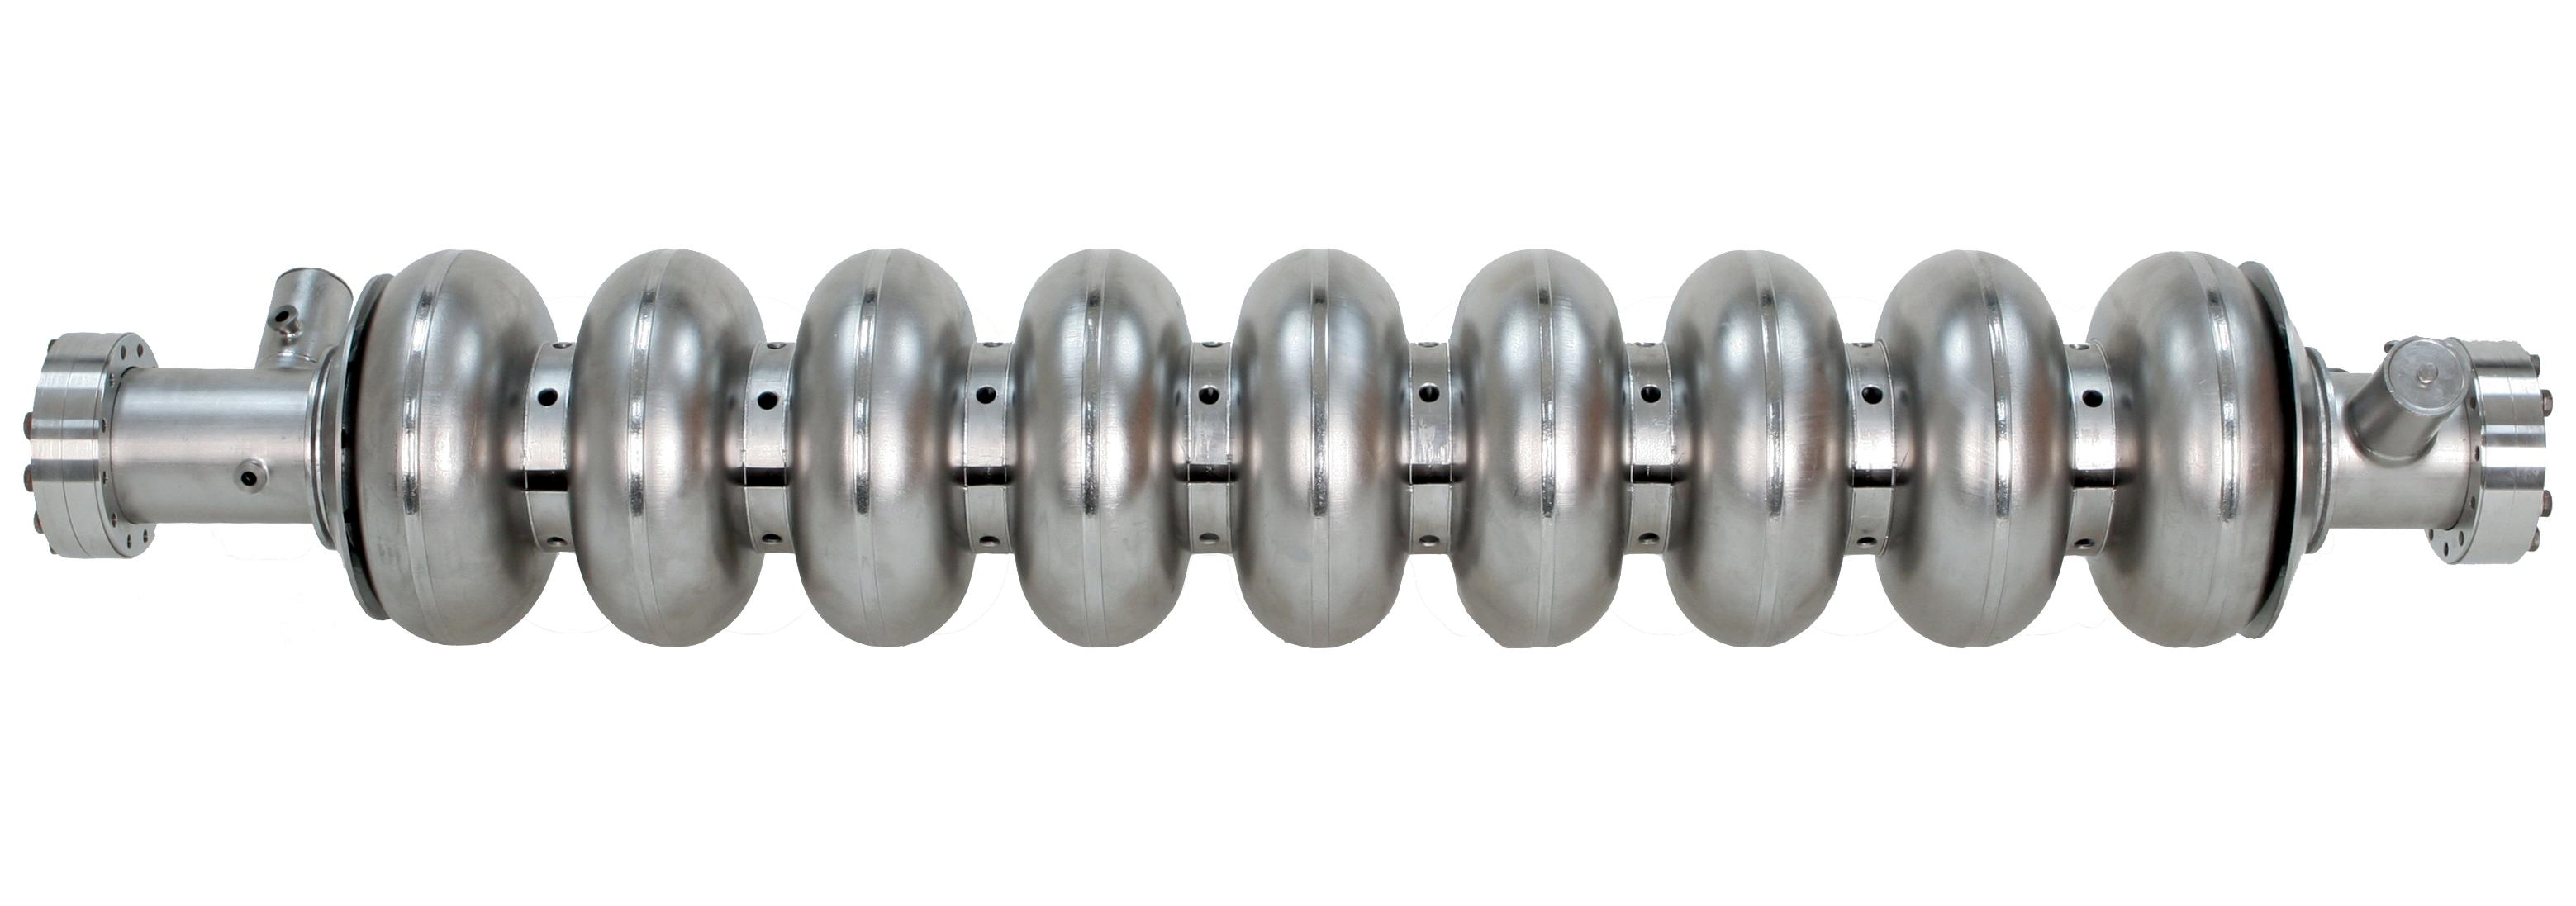
\includegraphics[width=0.95\textwidth]{graphics/Cavity.jpg}
    \caption{\sl External view of the ILC SCRF cavity.}
    \label{fig:ILCcavity}
  }
\end{figure}

\textit{The beam delivery system} is responsible for transporting electrons and positrons from the main high-energy linacs to the interaction point (IP). These systems monitor and focus the electron and positron beams to meet the luminosity requirements and after the collision it transports the residual particles to the beam dumps. 
The beams cross each other at 14\,mrad angle, which provide enough space for separate extraction lines. 

The design of ILC detector hall and beam delivery systems allow hosting of two experiments, SiD and ILD, sharing one interaction point using a push-pull approach. 
%Both detectors are designed as multi-purpose detectors, developed for a wide physics program. 

        \begin{landscape}
        \begin{table}
        \begin{center}
        \begin{tabular}{|lcc|c|c|c|c|c|c|}
                \hline
                Center-of-mass energy &$\sqrt{s}$ &GeV  			& 250 & 350 & 500 & upgrade 1000 \\ 
                Collision rate &$f_{\text{rep}}$ &Hz  				& 5 & 5 & 5 & 4 \\ 
                Electron linac rate &$f_{\text{linac}}$ &Hz  		& 10 & 5 & 5 & 4 \\ 
                Number of bunches &$n_b$ &							& 1,312 & 1,312 & 1,312 & 2450 \\ 
                Bunch population &$N$ &$\times 10^{10}$ 			& 2 & 2 & 2 & 1.74 \\ 
                Main linac average gradient &G$_{\text{av}}$ &MV/m  & 14.7 & 21.4 & 31.5 & 38.2 \\  \hline

                RMS bunch length &$\sigma_{\text{z}}$ &mm 			& 0.3 & 0.3 & 0.3 & 0.25 \\ 
                Electron RMS energy spread &$\Delta p/p$ &\%  		& 0.19 & 0.16 & 0.12 & 0.08 \\ 
                Positron RMS energy spread &$\Delta p/p$ &\%  		& 0.15 & 0.1 & 0.07 & 0.04 \\ 
                Electron polarization &$P_-$ &\%  					& 80 & 80 & 80 & 80 \\ 
                Positron polarization &$P_+$ &\%  					& 30 & 30 & 30 & 20 \\ 
                IP RMS horizontal beam size &$\sigma_{\text{x}}*$ &nm& 729 & 683 & 474 & 481 \\ 

                %(without traveling focus)  &&& & & & \\
                IP RMS vertical beam size &$\sigma_{\text{y}}*$ &nm  & 7.7 & 5.9 & 5.9 & 2.8 \\ \hline
                Luminosity &$\mathcal{L}$ &$\times 10^{34}$\,cm$^{-2}s^{-1}$ & 0.75 & 1.0 & 1.8 & 3.6 \\ 
                Fraction of luminosity in top 1\% &$\mathcal{L}_{0.01}/\mathcal{L}$ & & 87.1\% & 77.4\% & 58.3\% & 59.2\% \\ 
                Average energy loss &$\delta E_{\text{BS}}$&  & .97\% & 1.9\% & 4.5\% & 5.6\% \\  \hline
				Number of pairs per bunch crossing &$N_{pairs}$ &$\times 10^3$ & 62.4 & 93.6 & 139.0 & 200.5 \\ 
                Top pair energy per bunch crossing &$E_{pairs}$ &TeV & 46.5 & 115.0 & 344.1 & 1338.0 \\ \hline
        \end{tabular}
        \end{center}
        \caption{Parameters of the ILC, as given in~\cite{bib:ILC}. }
        \label{tab:ILCparam}
        \end{table}
        \end{landscape}

%%%%%%%%%%%%%%%%%%%%%%%%%%%%%%%%%%%%%%%%%%%%%
%%%%%%%%%%%%%%%%%%%%%%%%%%%%%%%%%%%%%%%%%%%%%
%%%%%%%%%%%%%%%%%%%%%%%%%%%%%%%%%%%%%%%%%%%%%


\subsection{Detector requirements and motivation}

Realization of the ILC physics program require significant advances in the detector performance. 

%Jet energy resolution
One of the main challenges for detector hardware and reconstruction software is the high-precision jet energy measurement, which is crucial, for example, for top mass measurements. This and many other studies require 3-4\%  energy resolution for 100\,GeV jets.
% ---> PFA
The Particle flow algorithms, which are able to reconstruct individual particles inside jets, have been developed to fit this requirement. 
% ---> SiW ECAL
A successful implementation of this technique needs a highly granular electromagnetic and hadron calorimeters.
The Particle flow technique also requires thick calorimeters for full electromagnetic and hadron shower absorption.

% Charged track resolution 
Higgs recoil mass measurement using $e^+e^- \to Z^0H$ process, requires high precision measurements of charged tracks, left by lepton pair from $Z^0$ boson decay. The goal for tracking subdetectors and magnetic solenoid is a momentum resolution for charged tracks $\Delta p/ p^2 \approx 5 \cdot 10^{-5}$\,GeV$^{-1}$.

% Impact parameter resolution
The reconstruction of top and Higgs decays into $b$-quark and $c$-quark pairs, as well as many other processes, require a high-precision measurements of track impact parameters by vertex detectors. To achive the targeted flavour tagging performance, the required impact parameter resolution depending on track momentum $p$ and track polar angle $\theta$ should be $\sigma_b < 5  \oplus 10/p/\sin^{4/3}\theta$\,$\mu$m.

% ---> Low material deposit
To fit these requirements, all tracking devices should have minimal material budget to minimize particle scattering processes, therefore, a lightweight detectors, such as silicon or gaseous readout devices are preferred.

% Power pulsing
The ILC beam parameters allow to power off many detector subsystems between bunch trains, which reduces heat production and need for active cooling. This method is called power pulsing, and allows reducing the insensitive volumes and reduce material budget for inner trackers, which could be taken by active cooling systems. 

%%%%%%%%%%%%%%%%%%%%%%%%%%%%%%%%%%%%%%%%%%%%%
%%%%%%%%%%%%%%%%%%%%%%%%%%%%%%%%%%%%%%%%%%%%%
%%%%%%%%%%%%%%%%%%%%%%%%%%%%%%%%%%%%%%%%%%%%%

\subsection{The International Large Detector}


The International Large Detector (ILD) is a high precision multi-purpose detector concept, designed to meet the physics goals.
The ILD design is a result of physics driven approach in developing of detector concept by a wide scientific community. 

The ILD Detector Baseline Design (DBD) is the only approved ILD model within the ILC community, which is optimized for best resolution and a flexibility towards higher center-of-mass energies
up to the TeV range.
The major ILD subdetectors, ordered by distance from the interaction point outside, are the following:
\begin{itemize}
\item Vertex Detector (VXD) and Forward Tracking Disks (FTD) are the innermost detectors of ILD, which serve to measure impact parameters of particles;
\item Silicon Inner Tracker (SIT) is used to connect track segments from VXD and TPC;
\item Time Projection Chamber (TPC) serves for charge and momentum reconstruction and particle identification
\item Endplate of the TPC (ETD) and Silicon External Tracker (SET) provide a connection between tracks and calorimeter energy depositions 
\item High granular Silicon Tungsten Electromagnetic Calorimeter (\ecal) is used to measure and tag electromagnetic energy depositions;
\item Highly segmented Hadronic Calorimeter (HCAL) provides reconstruction and identification of hadrons;
\item Superconducting solenoid creates 3.5~T magnetic field;
\item Tail Catcher and Muon Tracker (TCMT) serves for muon identification and hadron energy measurement.
\end{itemize}
The schematic layout of main ILD subsystems is given in Fig.~\ref{fig:ILDScheme}.


\begin{figure}
\centering
\begin{subfigure}{0.5\textwidth}
    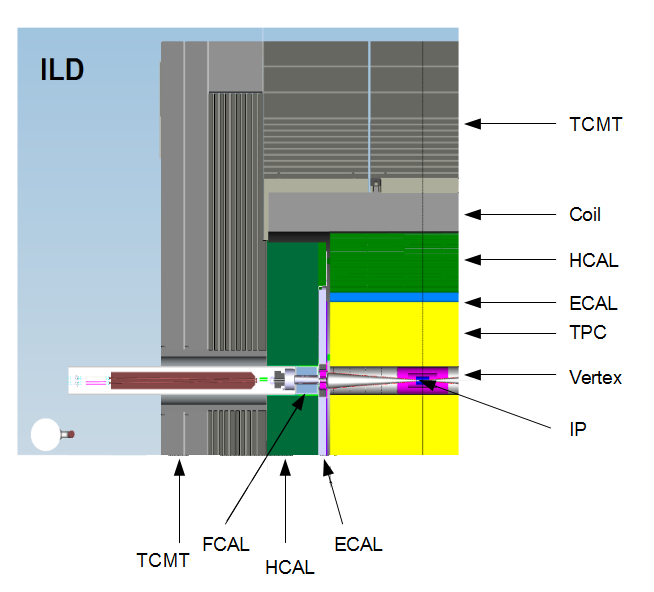
\includegraphics[width=0.95\textwidth]{graphics/ILD.png}

\end{subfigure}% 
  \begin{subfigure}{0.5\textwidth}
\centering
    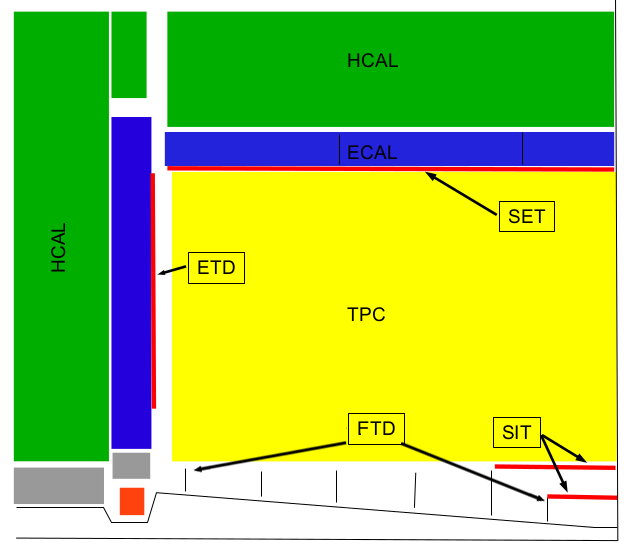
\includegraphics[width=0.9\textwidth]{graphics/ILDtracking.png}

\end{subfigure}
    \caption{\sl Left: Schematic view of the ILD. Right: Zoom in the inner detectors.}
    \label{fig:ILDScheme}
\end{figure}

% L* models
%However, there are many variations of the baseline model in order to achieve a better physics performance, push-pull synchronization with SiD or cost-performance optimization. 


%%%%%%%%%%%%%%%%%%%%%%%%%%%%%%%%%%%%%%%%%%%%%
%%%%%%%%%%%%%%%%%%%%%%%%%%%%%%%%%%%%%%%%%%%%%
%%%%%%%%%%%%%%%%%%%%%%%%%%%%%%%%%%%%%%%%%%%%%
\subsubsection{Particle flow reconstruction technique}
The ILD concept is designed to meet all requirements for application of the Particle Flow Algorithms (PFA) for physics analysis. 

The PFA allows reconstruction of individual particles, even inside jets, which significantly improves the jet energy resolution, by relying on information from inner tracker and calorimeters.
These algorithms operate Particle Flow Objects (PFO), that are reconstructed using hits in the tracking devices and calorimeters. 

\begin{figure}
{\centering
    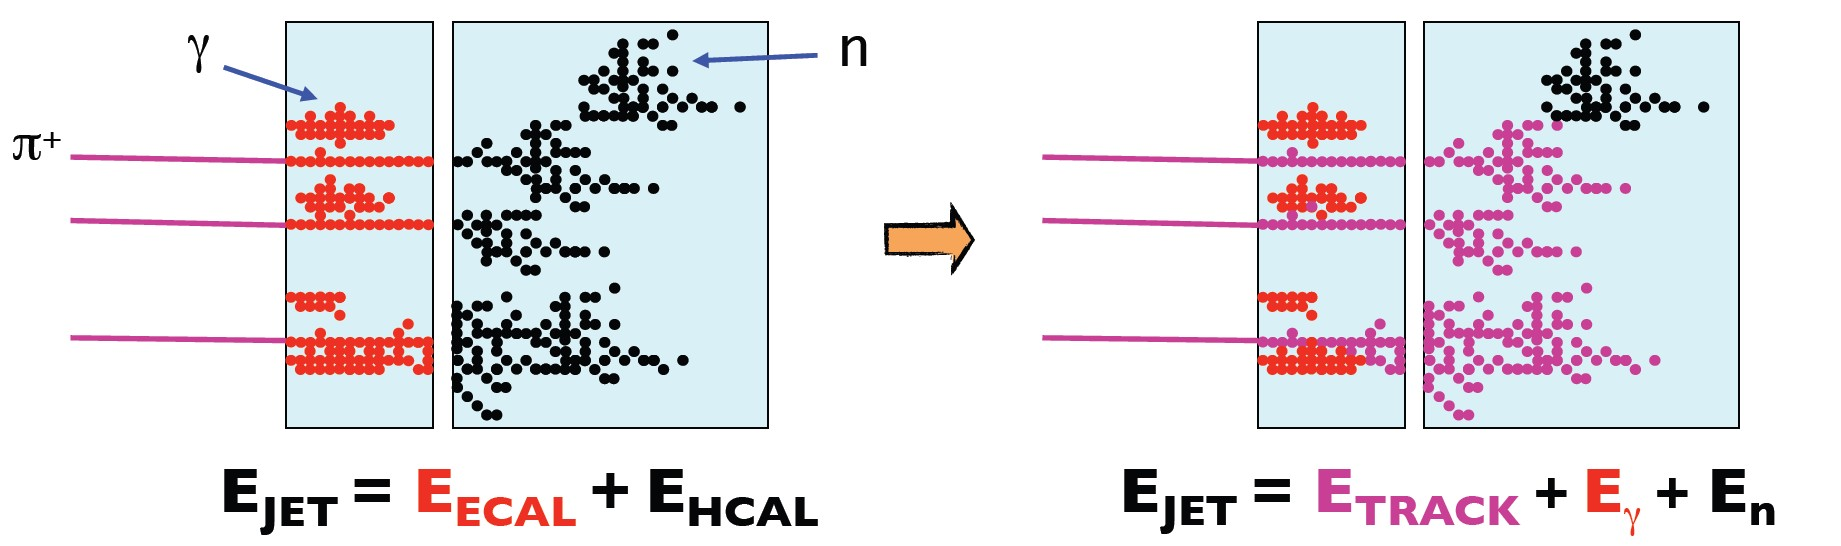
\includegraphics[width=0.95\textwidth]{graphics/calirometry_traditional_new.jpg}
    \caption{\sl Left: Illustration of a jet energy estimation, which is based only on the calorimeter information. Right: Illustration of the Particle flow algorithms, which measure jet energy as a sum of charged and neutral particle energies.}
    \label{fig:PFAillustration}
  }
\end{figure}
%Tracking

First stage of the PFO formation is an individual track reconstruction using tracker information. Tracks have the form of a helix, as a consequence of magnetic field influence on charged particles.  The most common algorithm used is Kalman Filter.
%clusterization
Then, the energy depositions in the ECAL and HCAL are organized into topological clusters, which are grouped into showers, that correspond to the individual interactions of final-state particles. In general case, the showers, left by hadrons, differ from photon or electron clusters. The granularity of the calorimeter plays an essential role in the clusterization process. High-granular calorimeters are able to separate close-by energy depositions, left by different particles. The illustration of Particle flow process is given in Fig.~\ref{fig:PFAillustration}.

Typically, the PFA creates objects of the following types:
\begin{itemize}
\item Muons have a reconstructed track and track-like energy depositions in ECAL and HCAL, and hits in TCMT;
\item Photons have a compact neutral cluster in ECAL without a connected track;
\item Electrons are reconstructed as a compact cluster in ECAL with an associated track;

\item Neutral hadrons (neutrons, neutral kaons, etc.) appear as a hadronic cluster, that starts from ECAL and continues to HCAL and TCMT;
\item Charged hadrons (protons, charged kaons, etc.) appear as track, connected to an hadronic cluster.
\end{itemize}

After creating of PFOs, one can use different algorithms like vertex detection, jet clustering, particle identification, flavor-tagging algorithms, etc.

One of the fundamental characteristics of the PFA performance is jet energy resolution shown for ILD concept in Fig.~\ref{fig:ILCjetrms}, which shows that the detector model is able to meet the requirement of 3-4\% resolution.

\begin{figure}[H]
{\centering
    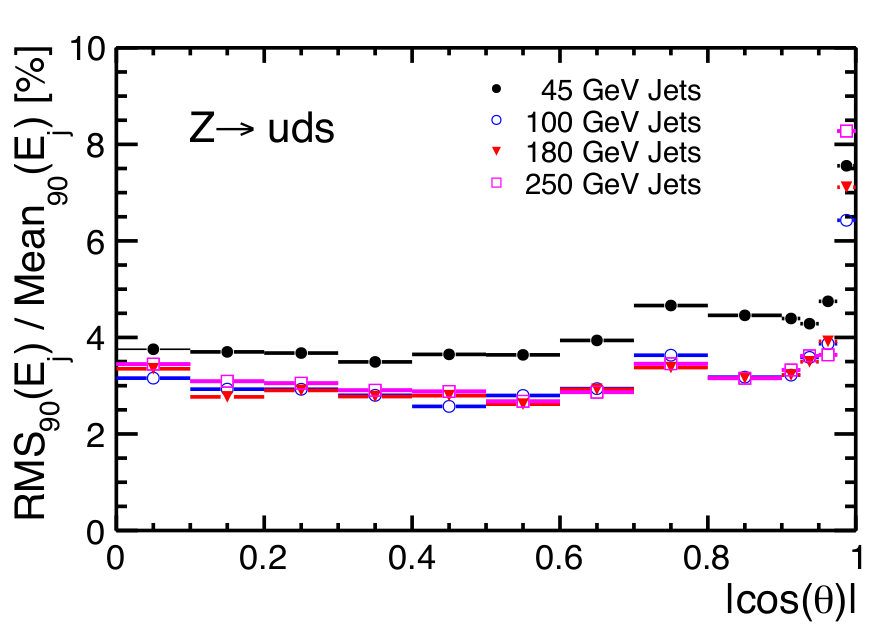
\includegraphics[width=0.55\textwidth]{graphics/ILCjetrms.png}
    \caption{\sl Fractional jet energy resolution plotted versus $|\cos\theta|$ where $\theta$ is the polar angle of the thrust axis of the event.}
    \label{fig:ILCjetrms}
  }
\end{figure}


%The PFA technique was successfully applied in CMS experiment at LHC.% CMS

%%%%%%%%%%%%%%%%%%%%%%%%%%%%%%%%%%%%%%%%%%%%%
%%%%%%%%%%%%%%%%%%%%%%%%%%%%%%%%%%%%%%%%%%%%%
%%%%%%%%%%%%%%%%%%%%%%%%%%%%%%%%%%%%%%%%%%%%%

\subsubsection{Vertex Detector}
The Vertex Detector of ILD serves to reconstruct position of primary interaction point (IP) and detect tracks with an offset to the IP and organize them into secondary or ternary vertices. The secondary vertices are created by high energy particles with a relatively short lifetime, like B mesons, D mesons or $\tau$ leptons. These particles appear in major decay modes of the Higgs boson or top quark. Therefore, the accurate measurement of track offsets, efficient tagging of $b$- and $c$-quark jets is crucial for top and Higgs physics program. %Another important role of VXD is to reject beam background particles, which requires fast timing of readout devices.

To fulfill required precision, the VXD is designed to have first layer at 16\,mm radius from the IP, \~3\,$\mu$m spatial resolution on track impact parameter and a low material budget of the device. To avoid installation of liquid cooling, the ILD Vertex Detector should also have a low power consumption.

The baseline design of VXD consist of three cylindrical double layers with pixel sensors as readout devices. The VXD layer characteristics are given in Table~\ref{table:ILCvtxparam}.
The VXD layout and its mechanical support is shown in Fig.~\ref{fig:ILCvtxsupport}. 

        \begin{table}[H]
        \begin{center}
        \begin{tabular}{l c c c c c}
        \hline
        			& $R$ (mm) & $|z|$ (mm) & $|\cos\theta|$ & $\sigma$ ($\mu$m) & Readout time ($\mu$m)\\
        \hline
            Layer 1 & 16 & 62.5 & 0.97 & 2.8 & 50 \\
            Layer 2 & 18 & 62.5 & 0.96 & 6 & 10 \\
        \hline
            Layer 3 & 37 & 125 & 0.96 &  4 & 100 \\
            Layer 4 & 39 & 125 & 0.95 &  4 & 100 \\
        \hline
            Layer 5 & 58 & 125 & 0.91 &  4 & 100 \\
            Layer 6 & 60 & 125 & 0.9 &   4 & 100 \\
        \hline
        \end{tabular}
        \end{center}
        \caption{\sl Parameters of the ILC vertex detector system, as given in~\cite{bib:ILC}. }
        \label{table:ILCvtxparam}
        \end{table}

\begin{figure}
\centering

    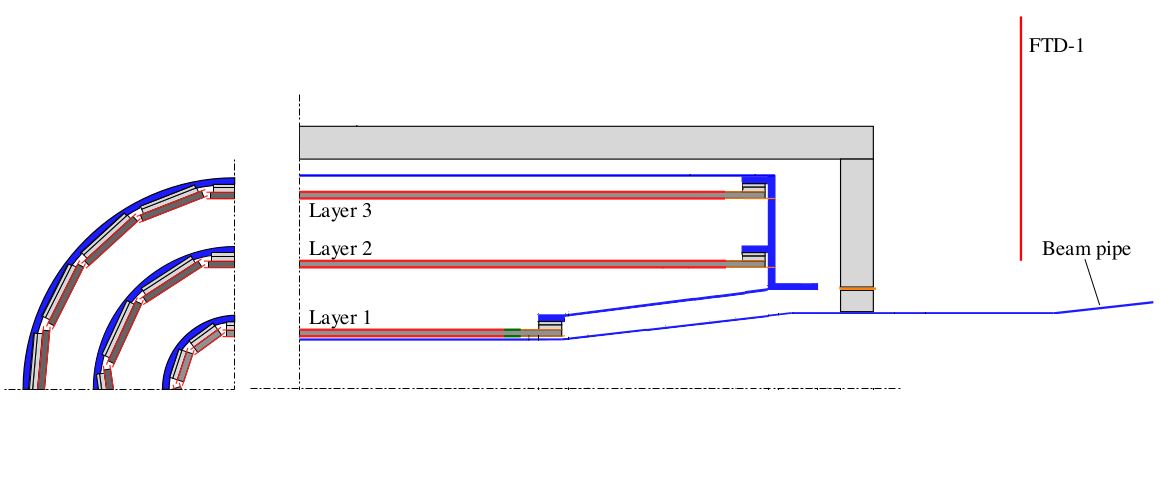
\includegraphics[width=0.9\textwidth]{graphics/ILCvtxsupport.png}
    \caption{\sl Mechanical support structure of ILD vertex detector.}
    \label{fig:ILCvtxsupport}


\end{figure}

Currently, three readout device technology are considered: CMOS Pixel Sensors (CPS), Fine Pixel CCD (FPCCD) and Depleted Field Effect Transistor (DEPFET).
All three technologies are able to provide sensors with up to 50\,$\mu$m thickness and a timing resolution of $\leq 10\mu$s. 

%%%%%%%%%%%%%%%%%%%%%%%%%%%%%%%%%%%%%%%%%%%%%
%%%%%%%%%%%%%%%%%%%%%%%%%%%%%%%%%%%%%%%%%%%%%
%%%%%%%%%%%%%%%%%%%%%%%%%%%%%%%%%%%%%%%%%%%%%

\subsubsection{Forward Tracking Discs}

The ILD forward tracking region consist of seven tracking disks  placed between the beam pipe and the TPC. The first two are equipped with pixel sensors to provide good impact parameter resolution, the other five have silicon strips as readout devices and serve for momentum and charge reconstruction. The layout of the Forward Tracking Discs is described in Table~\ref{table:ILCftdparam}. 

        \begin{table}[H]
        \begin{center}
        \begin{tabular}{l c c c c c }
        \hline
        			& $R$ (mm) & $|z|$ (mm) & $|\cos\theta|$ & $\sigma$ ($\mu$m) & Material (\%)\\
        \hline
            Layer 1 & 39-164 & 220 &  0.985-0.802 &  & 0.25-0.5 \\
            Layer 2 & 50-164 & 371 &  0.991-0.914 & 3-6 & 0.25-0.5 \\
        \hline
            Layer 3 & 70-308 & 645 &  0.994-0.902 &   & 0.65 \\
            Layer 4 & 100-309 & 1046 & 0.994-0.959 &   & 0.65 \\
            Layer 5 & 130-309 & 1447 & 0.995-0.998 &  7.0 & 0.65 \\
            Layer 6 & 160-309 & 1848 & 0.996-0.986 &    & 0.65 \\
            Layer 7 & 190-309 & 2250 & 0.996-0.990 &    & 0.65 \\
        \hline
        \end{tabular}
        \end{center}
        \caption{\sl Parameters of ILD Forward Tracking Disks system, as given in~\cite{bib:ILC}. }
        \label{table:ILCftdparam}
        \end{table}

%The main challenges of the FTD are 
Solenoidal magnetic field has a reduced influence on particles in the ILD forward region, thus a precise momentum measurement requires a low material budget and large lever arm. Even small amount of material before the first sensitive layer can disturb impact parameter precision. To archive the required performance, first two inner disks are implemented using high-granular pixels with around 3\,$\mu$m resolution and minimal material budget. As for Vertex detector, the similar technologies of readout devices are considered: CPS, FPCCD and DEPFET. Outer disks are equipped with AC coupled p-on-n fine-pitch microstrip silicon sensors.
%%%%%%%%%%%%%%%%%%%%%%%%%%%%%%%%%%%%%%%%%%%%%
%%%%%%%%%%%%%%%%%%%%%%%%%%%%%%%%%%%%%%%%%%%%%
%%%%%%%%%%%%%%%%%%%%%%%%%%%%%%%%%%%%%%%%%%%%%

\subsubsection{Time Projection Chamber}

The ILD central tracker is required to have low material budget, high precision, good timing resolution and have enough points for track reconstruction. Time Projection Chamber is the best device to fulfill all these requirements. 

TPC consist of an endplate, where the readout of the amplified signals takes place using custom-designed electronics, and a fieldcage, made from advanced composite materials. 
Charged particles, that enter the TPC, ionize the gas mixture inside the chamber. Under an influence of an electric field from fieldscage, the electrons from track ionization drift to a TPC endplate, equipped with detection devices. As a result, TPC can provide up to 224 points per track.
A general layout of ILD TPC is shown in Fig.~\ref{fig:ILCtpc}. 
\begin{figure}
{\centering
    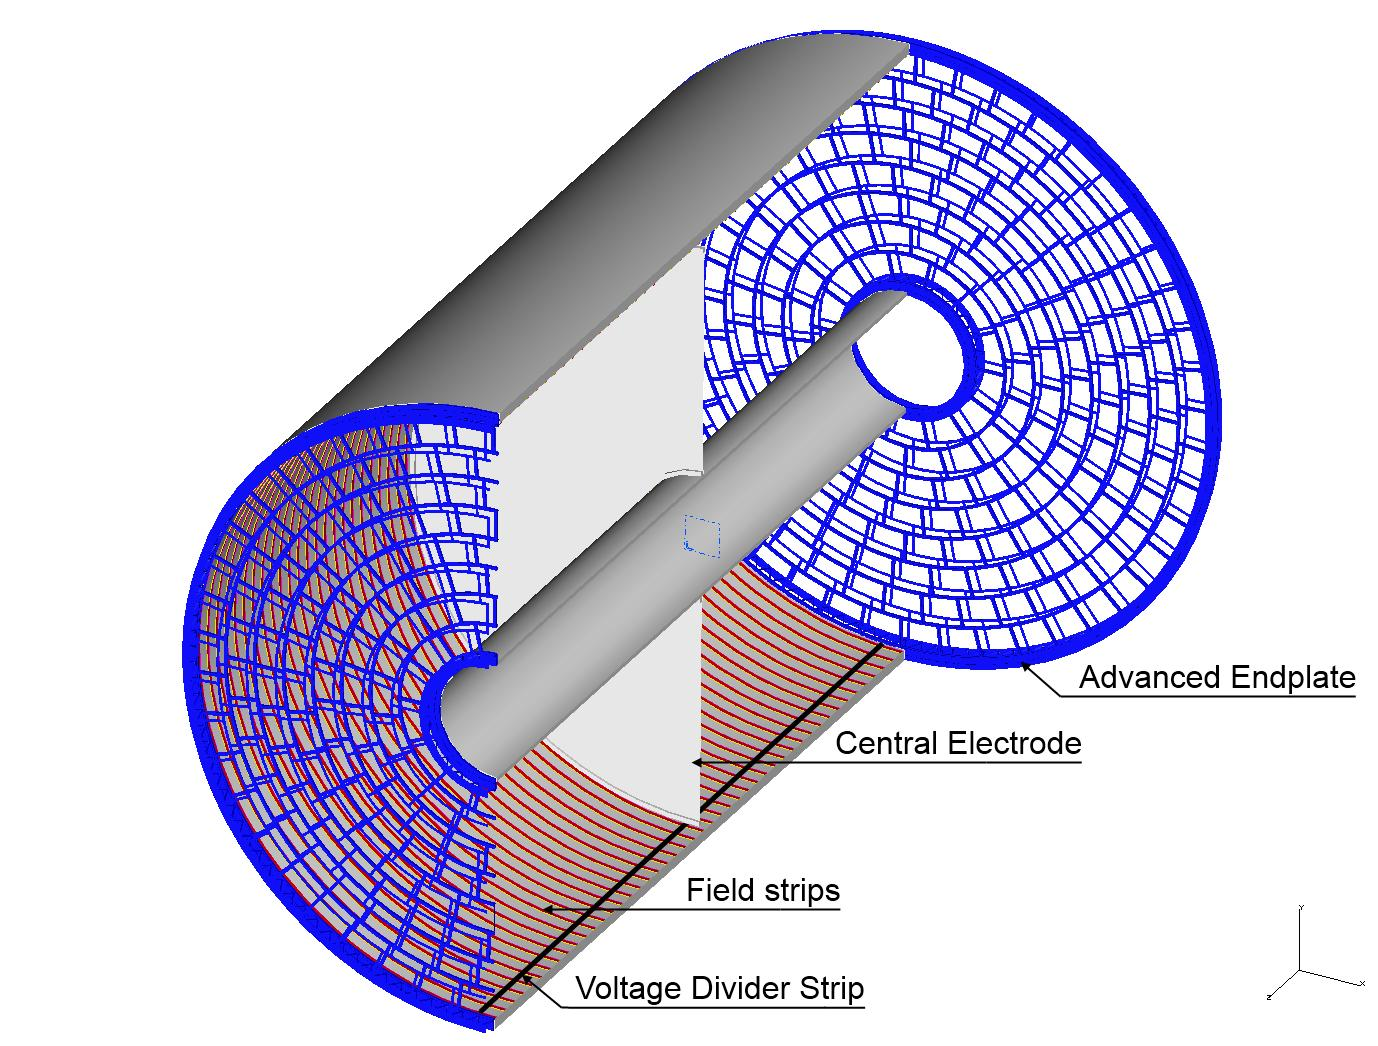
\includegraphics[width=0.55\textwidth]{graphics/ILCtpc.jpg}
    \caption{\sl Scheme of the TPC system showing the main parts of the device.}
    \label{fig:ILCtpc}
  }
\end{figure}

Currently, Micromegas and Gas Electron Multipliers are considered as detection methods. Both types of detection devices allow to measure energy deposition per particle track length $dE/dx$, which can be effectively used for particle identification (PID).

A detailed R\&D of TPC for ILD concept is provided by LCTPC collaboration.
%%%%%%%%%%%%%%%%%%%%%%%%%%%%%%%%%%%%%%%%%%%%%
%%%%%%%%%%%%%%%%%%%%%%%%%%%%%%%%%%%%%%%%%%%%%
%%%%%%%%%%%%%%%%%%%%%%%%%%%%%%%%%%%%%%%%%%%%%

\subsubsection{Other tracking detectors}
Silicon Inner Tracker, Silicon External Tracker and Endplate for TPC comprise Silicon Envelope of ILD and serve for time-stamping, TPC calibration and track segment synchronization. 
%The general scheme of the system is displayed in Fig.~\ref{fig:ILCtracking}.


SIT is located between Vertex Detector and TPC, it has two double-sided silicon strip layers, which provide necessary connection between VXD and TPC track segments. ETD and SET are realized with one double-sided layer of silicon strips, which provide a precise entry point of a charged track to the ECAL. The silicon envelope detectors use the same sensor type throughout the system.

The Silicon Envelope of ILD has been developed by the SiLC collaboration.
%%%%%%%%%%%%%%%%%%%%%%%%%%%%%%%%%%%%%%%%%%%%%
%%%%%%%%%%%%%%%%%%%%%%%%%%%%%%%%%%%%%%%%%%%%%
%%%%%%%%%%%%%%%%%%%%%%%%%%%%%%%%%%%%%%%%%%%%%

\subsubsection{Calorimeter System}

The Particle flow approach drives the calorimeter design. The high granular calorimeters of ILD can be used not only for a particle energy measurements, but also for a shower separation and particle identification. 

The principal role of ECAL in the PFA framework is photon reconstruction in presence of close-by particles. The device should be able to disentangle electromagnetic showers caused by photons or electrons from hadronic ones. Thus, high granularity in three dimensions is required. For these purposes ILD ECAL has a sandwich-like structure of 30 active readout layers with tungsten absorber layers in between. The total thickness of the absorber corresponds to 24 radiation lengths $X_0$ and 1 nuclear interaction length $\lambda$. The readout technology is silicon pin diodes of 5 $\times$ 5\,mm$^2$ size. This device is referred as \ecal. Another option for readout sensors is scintillator strips with silicon photomultipliers.

The hadronic calorimeter is designed to separate neutral and charged hadrons and precisely measure energy depositions of neutral hadrons. The HCAL has 42 sensitive layers with steel absorber in between. Two baseline readout options are considered, the scintillator-tile based AHCAL and the Glass Resistive Plate Chamber (GRPC) based SDHCAL.

CALICE collaboration made a detailed R\&D of ILD calorimeters, constructed and tested prototypes with different readout options. 
\ecal\ prototype by CALICE collaboration is described in Section~\ref{section:Ecal}.

%%%%%%%%%%%%%%%%%%%%%%%%%%%%%%%%%%%%%%%%%%%%%
%%%%%%%%%%%%%%%%%%%%%%%%%%%%%%%%%%%%%%%%%%%%%
%%%%%%%%%%%%%%%%%%%%%%%%%%%%%%%%%%%%%%%%%%%%%

\subsubsection{Outer part}

The outer part of ILD concept consist of superconducting solenoid and muon system / tail catcher. 

The superconducting coil surrounds the ILD calorimeters and creates an axial magnetic field of 3.5~T.

TCMT serves for magnetic flux confinement and, at the same time, it provides a measurement of residual energy depositions of hadronic showers and muon-tagging. Sensitive layers can be either scintillator strips or resistive plate chambers. 


